% !TeX TS-program = xelatex
\documentclass[twoside=false,DIV=14]{scrartcl}

\usepackage{arev} % order matters, putting this above allows FiraSans to override it for body text
\usepackage[sfdefault]{FiraSans}
\usepackage{inconsolata}
%\usepackage[fira]{fontsetup}
\usepackage{scrlayer-scrpage}
\renewcommand{\titlepagestyle}{scrheadings}
\usepackage{graphicx}
\usepackage{blindtext}
\usepackage{wrapfig}
\usepackage{tabularx}
\usepackage{hyperref}
\usepackage{listings}
\usepackage{tikz}
\usepackage{amsmath}
\usepackage[many]{tcolorbox}

\usepackage{xcolor,sectsty}
\definecolor{blackish}{RGB}{56,58,54}
\definecolor{redish}{RGB}{109,41,49}
\definecolor{red}{RGB}{152,41,50}
\definecolor{orangeish}{RGB}{188,71,0}
\definecolor{blueish}{RGB}{25,33,139}
\subsubsectionfont{\color{blackish}}
\subsectionfont{\color{blackish}}
\sectionfont{\color{blackish}}

\lohead{\color{red} COMP3000 Programming Languages}
\rohead{
\includegraphics[width=0.5cm]{../logo.jpg}}

\setkomafont{author}{\sffamily \small}
\setkomafont{date}{\sffamily \small}

\DeclareOldFontCommand{\bf}{\normalfont\bfseries}{\mathbf}
\DeclareOldFontCommand{\tt}{\normalfont\ttfamily}{\texttt}

\lstset{basicstyle=\ttfamily}


\date{}
\newtcolorbox{aside}[1][]{
  title=Aside,
  width=0.3\textwidth,
  fonttitle=\bfseries,
  breakable,
  fonttitle=\bfseries\color{black},
  colframe=blueish!80,
  colback=blueish!2
  #1}

\newtcolorbox{note}[1][]{
  title=Note,
  width=\textwidth,
  fonttitle=\bfseries,
  breakable,
  fonttitle=\bfseries\color{black},
  colframe=orangeish!80,
  colback=orangeish!2
  #1}

\newtcolorbox{hint}[1][]{
    title=Hint,
    width=\textwidth,
    fonttitle=\bfseries,
    breakable,
    fonttitle=\bfseries\color{white},
    colframe=blueish!80,
    colback=blueish!2
    #1}

\newtcolorbox{todo}[1][]{
  title=!! TODO !!,
  width=\textwidth,
  fonttitle=\bfseries,
  breakable,
  fonttitle=\bfseries\color{white},
  colframe=red!80,
  colback=red!2
  #1}
  
\providecommand{\tightlist}{%
  \setlength{\itemsep}{0pt}\setlength{\parskip}{0pt}}

\newcommand{\swaplr}{swap L and R}
\newcommand{\nrpp}{no, so R++}
\newcommand{\ylpp}{yes, so L++}
\newcommand{\isrp}{is $a[R] <$ pivot? }

\title{\color{redish} \vspace{-2em}Week 5 Workshop: Advanced Sorting}

\begin{document}
{\color{blackish}\maketitle}\vspace{-2em}%\input{proposal.inc}
\begin{itemize}
    \item[$\cdot$] {\bf Resources:}\begin{itemize}
    \item  Week 4  Code Bundle.
    \end{itemize}
    \item[$\cdot$] {\bf To submit this week's work:} Submit your solution to Exercise \ref{sec:submission} to your teacher in class.  You should hand in a single piece of paper with your solution on it.  Be sure you include your name, student number, and the week number in the top-right of your submission.
\end{itemize}

\part*{Exercises}

\section{Merge Sort: Tracing - Submission}
\label{sec:submission}
\begin{note}
We have given you some tracing styles for merge sort (the whole sort, and the merge step).  We do encourage you to use those trace styles because we think they are good. However, you \emph{are} free to use whatever style works for you.  Also note that if the given traces don't make sense to you, watch the lecture video for that topic where the tracing style is explained.
\end{note}
Do a \emph{high-level} trace of merge sort of the following unsorted array:
\begin{lstlisting}[language=java]
int [] array = {4,1,3,5};
\end{lstlisting}
\subsection{Trace the merge}
Now add a more detailed trace of \emph{just the merge step} that occurred when the sorted subarrays \verb|{1,4}| and \verb|{3,5}| were merged.

\section{Merge Sort: Another Trace}
Do the same thing as exercise \ref{sec:submission} for the following array:
\begin{lstlisting}[language=java]
char[] array = {'w','o','l','l','y','i','b'};
\end{lstlisting}

\section{Merge Sort: Match the trace}
Below is a trace of merge sort for the following array.  Note the purple parts are not part of the trace, they are part of this question.
\begin{lstlisting}[language=java]
char[] array = {'s','o','t','a','l','m','y','x','w'};
\end{lstlisting}
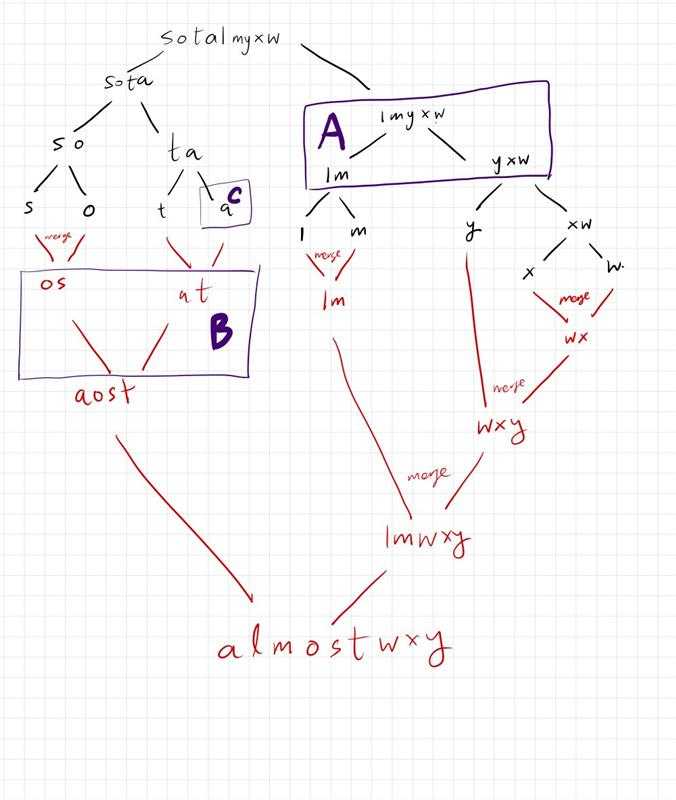
\includegraphics[width=0.8\textwidth]{sort_trace_plus.jpeg}

Your job is to work out exactly which lines of code are executing at each of the labelled parts of the trace, i.e $A$, $B$, and $C$.

\begin{lstlisting}[language=java,numbers=left]
public static char[] sort(char[] unsorted){
    if (unsorted.length == 1)
        return unsorted;
    int    mid   = unsorted.length/2;
    char[] left  = sort(Arrays.copyOfRange(unsorted, 0, mid));
    char[] right = sort(Arrays.copyOfRange(unsorted, mid, unsorted.length));
    return merge(left, right);
}    
\end{lstlisting}

\subsection{Zoom in on merge}
Here is the trace of the merge just where \verb|{'a','l','o','s','t'}| is merging with \verb|{'m','w','x','y'}|.  Your job is to identify \emph{exactly} which lines of code are running at points $D$ and $E$ of the trace.

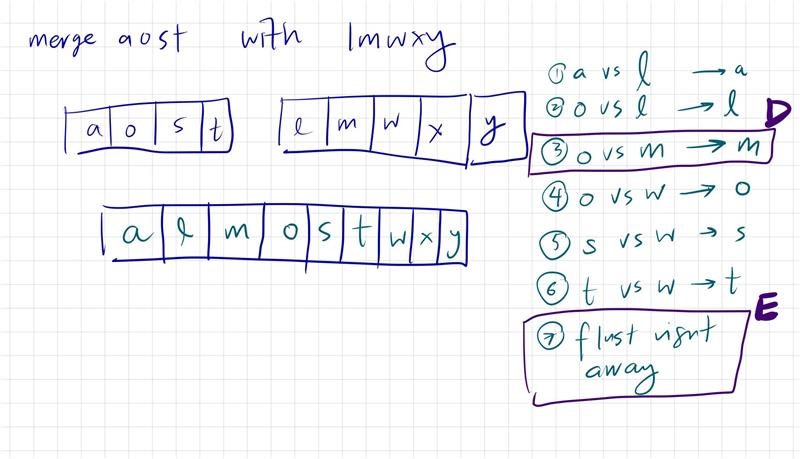
\includegraphics[width=\textwidth]{merge_trace_plus.jpeg}

\begin{lstlisting}[language=java,numbers=left]
public static char[] merge(char[] sorted_a, char[] sorted_b){
    char[] ret = new char[sorted_a.length + sorted_b.length];
    int i = 0;
    int j = 0;
    while (i < sorted_a.length && j < sorted_b.length){
        if(sorted_a[i] < sorted_b[j]){
            ret[i+j] = sorted_a[i];
            i++;
        } else {
            ret[i+j] = sorted_b[j];
            j++;                
        }
    }
    // flush the left
    while (i < sorted_a.length){
        ret[i+j] = sorted_a[i];
        i++;
    }

    // flush the right
    while (j < sorted_b.length){
        ret[i+j] = sorted_b[j];
        j++;
    }
    return ret;
}
\end{lstlisting}

\section{Merge Sort: Two ways}
Now rewrite the {\tt mergeSort}  and {\tt merge} functions so that they take an additional boolean parameter called {\tt upDown}. If  {\tt upDown} is set it {\tt true} then it performs an ascending sort, otherwise it performs a descending sort. Write a set of appropriate JUnit tests to check your programs.
    
\section{Quick Sort: Trace Partitioning}
The partition algorithm can seem like magic.  It's not obvious to me that all the conditions are right how can we just swap the partition at the end?  In this question we will just trace it out enough times to internalise an intuition.  There isn't a shortcut to just doing a heap of partitioning I'm afraid.

Trace the partition algorithm on the following full arrays (i.e. start is 0 and end is the last element of the array):
\begin{enumerate}
\item \verb+{2,1,3}+
\item \verb+{3,4,2,1,5}+
\item \verb|{5,4,6,3,7,2,8,1,9,0}|
\end{enumerate}
And when you are done with these, make up your own and trace them. Trace at least 10.  You can tell if your traces are right because if they are, the end array has all the elements less than the pivot on the left, all the elements more than the pivot on the right, and the pivot somewhere towards the middle.

\section{Quick Sort: Loop Invariant}
In your traces, identify the place where the loop starts and stops (i.e. the places where the loop invariant must hold).

Then check if the loop invariant we identified
\begin{quote}
    The items in \verb|a[1..L ]| are all strictly less than p, and the items in \verb|a[L+1..R-1]| are at least p.
\end{quote}

\begin{center}
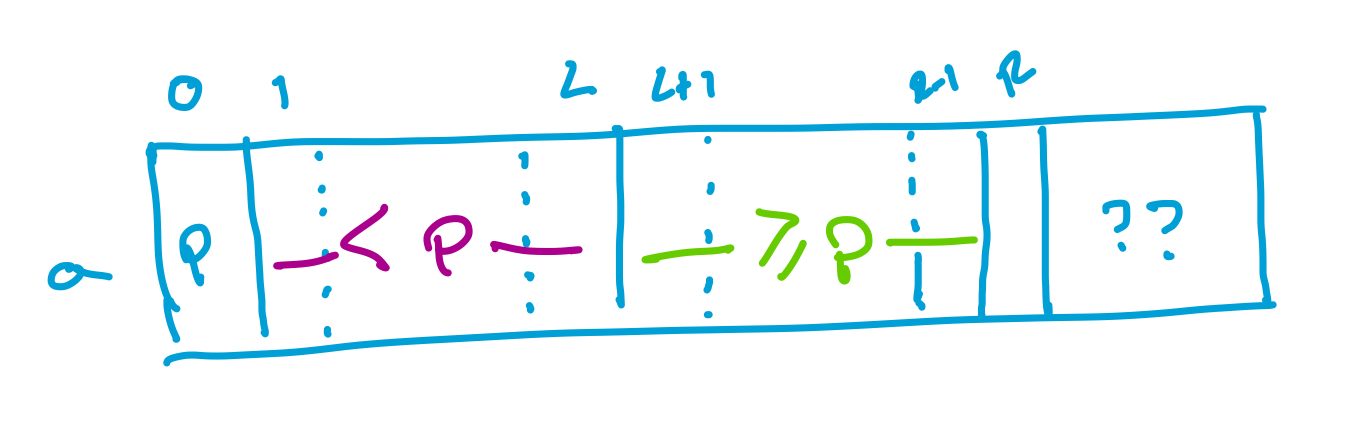
\includegraphics[width=0.6\textwidth]{pivot_invariant.jpeg}
\end{center}

is true in all those places.  When you have completed this, it should have helped you:
\begin{enumerate}
\item Understand the partition algorithm better.
\item Believe the partition algorithm is correct.
\end{enumerate}
    
\newpage\setcounter{section}{0}
\part*{Solutions}

\section{Merge Sort: Tracing}
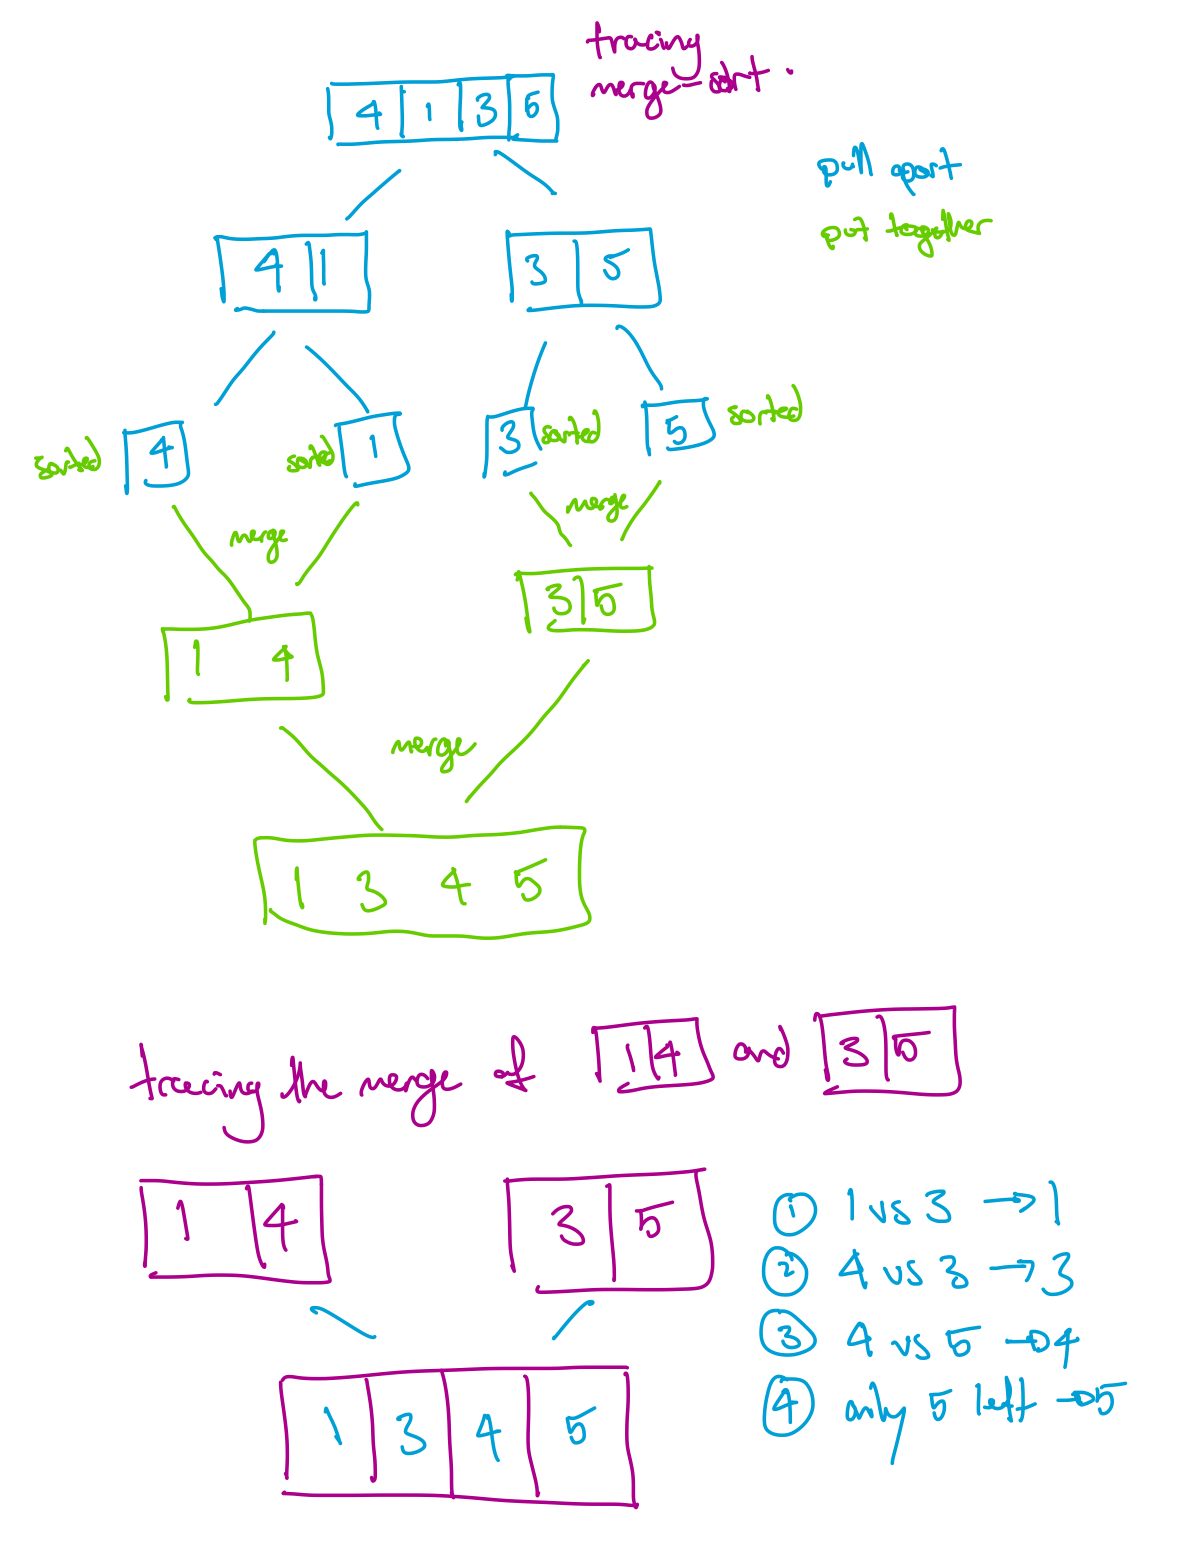
\includegraphics[width=0.7\textwidth]{small_merge_trace.jpeg}

\section{Merge Sort: Another Trace}
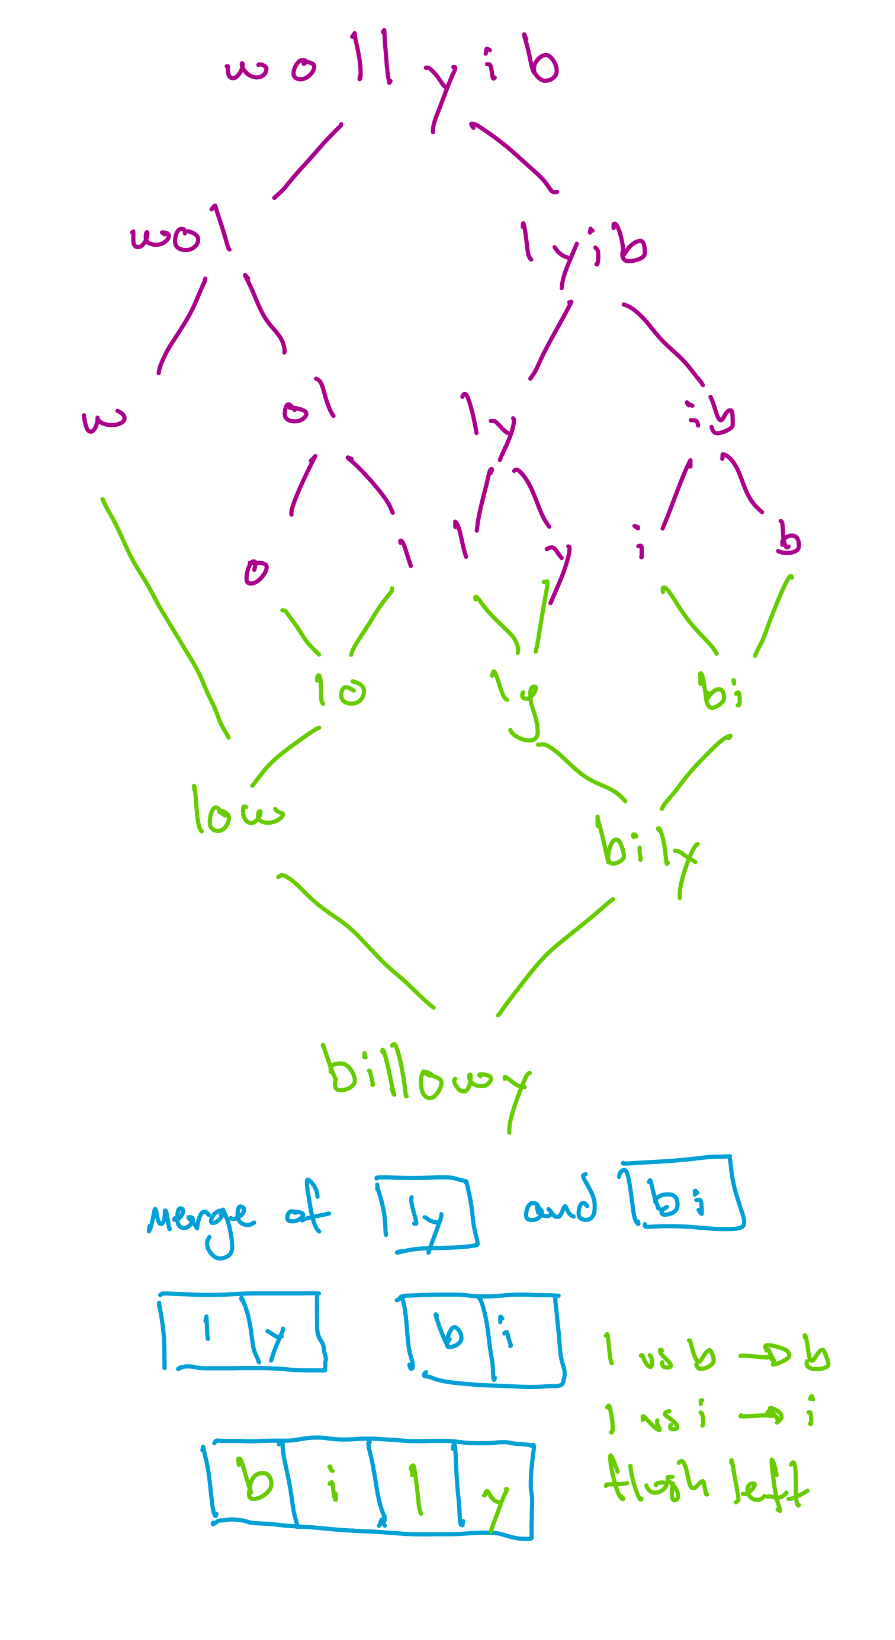
\includegraphics[width=0.6\textwidth]{mid_merge_trace.jpeg}

\section{Merge Sort: Match the Trace}
\begin{description}
\item[A] Lines 4--6
\item[B] Line 7
\item[C] Lines 1--2  
\end{description}

\subsection{Zoom in on merge}
\begin{description}
\item [D] Lines 9--12
\item [E] Lines 20--24
\end{description}

\section{MergeSort: Two Ways}
I only had to change a few places.  Here is a snippet of my solution showing the lines I needed to change:
\begin{description}
\item [line 1] I needed to add the extra parameter to \verb+sort+
\item [lines 5 and 6] I needed to pass that on to the recursive calls.
\item [line 7] The merge step needs to know as well.
\item [line 10] Thus I add a new parameter to \verb+merge+/
\item [lines 15 to 17] A cool trick here.  We pick from \verb+sorted_a+ whenever it is less that \verb|sorted_b| \emph{and} we are doing the normal ascending order.  However we also pick from \verb+sorted_a+ when it is greater than \verb|sorted_b| and we are doing descending order.  No other code needs to change!.
\end{description}
\begin{lstlisting}[language=java,numbers=left,basicstyle=\small]
public static char[] sort(char[] unsorted, boolean upDown){
    if (unsorted.length <= 1)
        return unsorted;
    int    mid   = unsorted.length/2;
    char[] left  = sort(Arrays.copyOfRange(unsorted, 0, mid), upDown);
    char[] right = sort(Arrays.copyOfRange(unsorted, mid, unsorted.length), upDown);
    return merge(left, right, upDown);
}

public static char[] merge(char[] sorted_a, char[] sorted_b, boolean upDown){
    char[] ret = new char[sorted_a.length + sorted_b.length];
    int i = 0;
    int j = 0;
    while (i < sorted_a.length && j < sorted_b.length){
        if((sorted_a[i] < sorted_b[j] && upDown)
            ||
            (sorted_a[i] > sorted_b[j] && !upDown)){
            ret[i+j] = sorted_a[i];
            i++;
        } else {
            ret[i+j] = sorted_b[j];
...
...
...
\end{lstlisting}

Here are the tests I wrote

{\small
\begin{lstlisting}
@Test
public void testBasics(){
    assertArrayEquals(sort(new char[]{}, true), new char[]{});
    assertArrayEquals(sort(new char[]{'b','a'}, true), new char[]{'a','b'});
    assertArrayEquals(sort(new char[]{'b','a','j'}, true), new char[]{'a','b','j'});
    assertArrayEquals(sort(new char[]{}, false), new char[]{});
    assertArrayEquals(sort(new char[]{'b','a'}, false), new char[]{'b','a'});
    assertArrayEquals(sort(new char[]{'b','a','j'}, false), new char[]{'j','b','a'});
    assertArrayEquals(sort(new char[]{'b','a','c','d','e','f','j','k','j'}, true),
                           new char[]{'a','b','c','d','e','f','j','j','k'});
    assertArrayEquals(sort(new char[]{'b','a','c','d','e','f','j','k','j'}, false),
                           new char[]{'k','j','j','f','e','d','c','b','a'});
}
\end{lstlisting}
}

\section{Trace Partition}
Since my handwriting is very ordinary my partition traces can be hard to follow.  Thus I've done them neatly here but remember, you should be doing yours on paper, not carefully typing them up.

\subsection{Tracing \lstinline|\{2,1,3\}|}
Just for this one, I've put the code on the left so you can more easily reference what is happening.
\noindent \begin{minipage}[t]{.5\textwidth}\vspace{0pt}\begin{lstlisting}[language=java] 
void partition(char[] a){
    char pivot = a[0];
    char L = 0;
    char R = 1;
    while(R <= a.length-1){
        if (a[R] < pivot){
            L++;
            swap(a,L,R);
            R++;
        } else {
            R++;
        }
    }
    swap(a,0,L);
}\end{lstlisting}\end{minipage}\begin{minipage}[t]{.5\textwidth} \vspace{0pt}
\begin{tabular}{lr}
    $[2|1|3]$         & get pivot, left, and right \\
    $[2_P^L|1^R|3]$   & start loop \\
                        & \isrp \\
                        & \ylpp \\
    $[2_P|1^{LR}|3]$   & \swaplr \\
    $[2_P|1^{LR}|3]$   & R++ \\
    $[2_P|1^L|3^R]$    & Repeat Loop \\
                       & \isrp \\
                        & \nrpp \\
     $[2_P|1^L|3]^R$    & Repeat Loop Failure \\
                        & swap 0 and L \\
    $[1|2|3]$    &  \\
    Success! & \\
\end{tabular}
\end{minipage}

\subsection{Tracing \lstinline|\{3,4,2,1,5\}|}
\begin{tabular}{lr}
    $[3|4|2|1|5]$         & get pivot, left, and right \\
    $[3_P^L|4^R|2|1|5]$   & start loop \\
                        & \isrp \\
                        & \nrpp \\
    $[3_P^L|4|2^R|1|5]$   & \isrp \\
       & \ylpp \\
    $[3_P|4^L|2^R|1|5]$   & \swaplr \\
    $[3_P|2^L|4^R|1|5]$    & R++ \\
    $[3_P|2^L|4|1^R|5]$    & \isrp \\
                        & \ylpp \\
    $[3_P|2|4^L|1^R|5]$    & \isrp \\
                        & \swaplr \\
    $[3_P|2|1^L|4^R|5]$    & R++ \\
    $[3_P|2|1^L|4|5^R]$     & Repeat Loop  \\
                        & \isrp \\
                        & \nrpp \\
    $[3_P|2|1^L|4|5]^R$ & Repeat Loop Failure \\
                        & swap 0 and L \\
    $[3_P|2|1^L|4|5]^R$   &  \\
    $[1|2|3|4|5]$ & \\
    Success! & \\
\end{tabular}

\subsection{Tracing \lstinline|\{5,4,6,3,7,2,8,1,9,0\}|}
\begin{tabular}{lr}
    $[5|4|6|3|7|2|8|1|9|0]$ & get pivot, left, and right \\
    $[5_P^L|4^R|6|3|7|2|8|1|9|0]$ & start loop \\
                        & \isrp \\
                        & \ylpp \\
    $[5_P|4^{LR}|6|3|7|2|8|1|9|0]$   & \swaplr \\
    $[5_P|4^{LR}|6|3|7|2|8|1|9|0]$   & L++ \\
    $[5_P|4^L|6^R|3|7|2|8|1|9|0]$   & repeat loop \\
    $[5_P|4^L|6^R|3|7|2|8|1|9|0]$   & \isrp \\
                                    & \nrpp \\
    $[5_P|4^L|6|3^R|7|2|8|1|9|0]$   & repeat loop \\
    & \isrp \\
    & \ylpp \\
    $[5_P|4|6^L|3^R|7|2|8|1|9|0]$   & \swaplr \\
    $[5_P|4|3^L|6^R|7|2|8|1|9|0]$   & R++ \\
    $[5_P|4|3^L|6|7^R|2|8|1|9|0]$   & repeat loop \\
       & \isrp \\
       & \nrpp \\
    $[5_P|4|3^L|6|7|2^R|8|1|9|0]$   & repeat loop \\
    & \isrp \\
    & \ylpp \\
    $[5_P|4|3|6^L|7|2^R|8|1|9|0]$   & \swaplr \\
    $[5_P|4|3|2^L|7|6^R|8|1|9|0]$   & R++ \\
    $[5_P|4|3|2^L|7|6|8^R|1|9|0]$   & R++ \\
    & \isrp \\
    & \nrpp \\
    $[5_P|4|3|2^L|7|6|8|1^R|9|0]$   & repeat loop \\
    & \isrp \\
    & \ylpp \\
    $[5_P|4|3|2|7^L|6|8|1^R|9|0]$   & \swaplr \\
    $[5_P|4|3|2|1^L|6|8|7^R|9|0]$   & R++ \\
    $[5_P|4|3|2|1^L|6|8|7|9^R|0]$   & repeat loop \\
    & \isrp \\
    & \nrpp \\
    $[5_P|4|3|2|1^L|6|8|7|9|0^R]$   & repeat loop \\
    & \isrp \\
    & \ylpp \\
    $[5_P|4|3|2|1|6^L|8|7|9|0^R]$   & \swaplr \\
    $[5_P|4|3|2|1|0^L|8|7|9|6^R]$   & R++ \\
    $[5_P|4|3|2|1|0^L|8|7|9|6]^R$   & repeat loop failure \\
    & swap 0 and L \\
    $[0|4|3|2|1|5|8|7|9|6]$ & \\
    Success! & \\
\end{tabular}

\subsection{Trace More}
I hope you did some more tracing, it matters for the next part.

\section{Quick Sort: Loop Invariant}
I am going to do this just for the third (largest) trace but you should do it for all yours.  I will add blue text at each point where the loop invariant needs to hold.  I then put the invariant in the line to help me check and a checkpoint if it holds.  Note that, in our notation, $a[L,R]$ where $L$ is greater than $R$ is an empty array.  I'm sorry, but I had to make it very small to fit.
\vspace{2em}

\newcommand{\invariant}{\color{blueish}$a[1..L] < p$ and $a[L+1..R-1] > p$ $\checkmark$}
{\tiny
\begin{tabular}{lr}
    $[5|4|6|3|7|2|8|1|9|0]$ & get pivot, left, and right \\
    $[5_P^L|4^R|6|3|7|2|8|1|9|0]$ & start loop \\
    \invariant & \\
                        & \isrp \\
                        & \ylpp \\
    $[5_P|4^{LR}|6|3|7|2|8|1|9|0]$   & \swaplr \\
    $[5_P|4^{LR}|6|3|7|2|8|1|9|0]$   & L++ \\
    $[5_P|4^L|6^R|3|7|2|8|1|9|0]$   &  \\
    \invariant & repeat loop \\
    $[5_P|4^L|6^R|3|7|2|8|1|9|0]$   & \isrp \\
                                    & \nrpp \\
    $[5_P|4^L|6|3^R|7|2|8|1|9|0]$   & \\
    \invariant & repeat loop \\
    & \isrp \\
    & \ylpp \\
    $[5_P|4|6^L|3^R|7|2|8|1|9|0]$   & \swaplr \\
    $[5_P|4|3^L|6^R|7|2|8|1|9|0]$   & R++ \\
    $[5_P|4|3^L|6|7^R|2|8|1|9|0]$   & \\
    \invariant & repeat loop \\
       & \isrp \\
       & \nrpp \\
    $[5_P|4|3^L|6|7|2^R|8|1|9|0]$   & \\
    \invariant & repeat loop \\
    & \isrp \\
    & \ylpp \\
    $[5_P|4|3|6^L|7|2^R|8|1|9|0]$   & \swaplr \\
    $[5_P|4|3|2^L|7|6^R|8|1|9|0]$   & R++ \\
    $[5_P|4|3|2^L|7|6|8^R|1|9|0]$   & R++ \\
    & \isrp \\
    & \nrpp \\
    $[5_P|4|3|2^L|7|6|8|1^R|9|0]$   & \\
    \invariant & repeat loop \\
    & \isrp \\
    & \ylpp \\
    $[5_P|4|3|2|7^L|6|8|1^R|9|0]$   & \swaplr \\
    $[5_P|4|3|2|1^L|6|8|7^R|9|0]$   & R++ \\
    $[5_P|4|3|2|1^L|6|8|7|9^R|0]$   & \\
    \invariant & repeat loop \\
    & \isrp \\
    & \nrpp \\
    $[5_P|4|3|2|1^L|6|8|7|9|0^R]$   & \\
    \invariant & repeat loop \\
    & \isrp \\
    & \ylpp \\
    $[5_P|4|3|2|1|6^L|8|7|9|0^R]$   & \swaplr \\
    $[5_P|4|3|2|1|0^L|8|7|9|6^R]$   & R++ \\
    $[5_P|4|3|2|1|0^L|8|7|9|6]^R$   & \\
    \invariant & repeat loop failure \\
    & swap 0 and L \\
    $[0|4|3|2|1|5|8|7|9|6]$ & \\
    Success! & \\
\end{tabular}
}
\newpage\setcounter{section}{0}
\part*{Self Study}

\section{Searching for better explanations}
Ask the internet to tell you how quick sort partition works.  You might find a video or your LLM might give you some text to read.  Is the answer you got compatible with what we are learning in COMP2010?

If so, very good, let me know if you think what you found is good and we can include it next year.

If not, what is going on?

\section{Merge Sort: Other variants}
Ask your resident LLM for a Java merge sort implementation.  Go back to the trace of
\begin{lstlisting}[language=java]
char[] array = {'s','o','y','a','l','m','y','x','w'};
\end{lstlisting} 
and try to match the LLM's code to the locations in the trace.  Do you find the LLM version easier or harder to understand?  Can you pinpoint any important differences in the operation of that version?

% \section{Merge Sort: Invariant}
% The \verb+merge+ part of merge sort has the following invariant which we discussed in lectures
% \begin{quote}
%     \verb|ret[0.. i + j - 1]| is the sorted merge of \verb+left[0..i-1]+ and \verb+right[0..j-1]+
% \end{quote}

% The form of trace we used for partitioning so far make it hard to check this.  Redo at least one of these traces in a form that lets you see that the invariant holds for at least a few loops.

\section{QuickSort: Variant}
The partition function used in QuickSort given in lectures requires a final swap of the pivot item p.   Now think of writing an alternative algorithm based on the following invariant.

\bigskip

\begin{quotation}
    ``All the items with index at least F but less than b are less than or equal to p;
            all the items with index greater than c, but no more than L have value at least p;
        A[b] == p"
        \end{quotation} 

\bigskip

Here F, L are the first and last indices of the array A, c is a counter that starts at L and should
be decremented, and b is an index that should always point to the position in the array whose item is p. Your algorithm should not require the final swap.
    
\begin{hint}
Draw a picture to help you envisage the shape of the invariant.
\end{hint}

\section{QuickSort: Alternative Domain}
Suppose the items in an array take one of three distinct values.  For example, the array could be:
    
\[
[0, 2, 1, 0, 0, 2, 1, 1, 2, 2, 2, 0, 1]~,
\]
    
where the values are all $0, 1, 2$.

Use the ideas from the 
partition function for quicksort to implement an algorithm that sorts the items in O(N), where N
is the length of the list. 
Write some JUnit tests to check your work.

\begin{hint}
Think of swapping elements out of the unknown region of the array.  Keep three sections of the list: an initial portion from index $0$ to index $f-1$ contains $0$'s; the portion from index $f$ to index $m-1$ contains $1$'s and the portion from index $b$ to $N-1$ contains $2$'s. Now think about swapping items in the unknown portion (from index $m$ to index $b-1$) into one of the three portions.
\end{hint}

\section{QuickSort: Search}
Let {\tt A} be an unsorted array of integers. Using the {\tt partition} function from {\tt quicksort} design an efficient algorithm which finds the {\tt  k}'th smallest item in {\tt A}. The k'th smallest item is the item which appears at index {\tt k} were the array to be completely sorted. Your solution should not sort the array entirely --- you can do it more efficiently than that.
    
\begin{hint}
Think about what would happen if your partition function returned the final position of the pivot $p$. Would you know the value of the {\tt k}'th smallest item?  if partition returned a value less than {\tt k} which part of the array would contain the {\tt k}'th smallest item?
\end{hint}
    
\section{All Sorts: Stability} 
A sort is said to be \emph{stable} if whenever two elements have the same value, then they must appear in the same order in the output as in the input. State which of {\tt mergeSort} and {\tt quickSort} are stable. In the case of the unstable ones, give an example.
    
\newpage\setcounter{section}{0}
\part*{Self Study Solutions}
\section{Quick Sort: Searching for better explanations}
CoPilot told me
\begin{quote}
    \textbf{Detailed Steps of Partitioning:}

    Initialization: Start with two pointers, one at the beginning (left) and one at the end (right) of the array.

    Move Pointers:
    \begin{itemize}
        \item Increment the left pointer until you find an element greater than or equal to the pivot.
        \item Decrement the right pointer until you find an element less than or equal to the pivot.
    \end{itemize}
    Swap Elements: If the left pointer is still less than or equal to the right pointer, swap the elements at these pointers. Then, move the pointers inward (left pointer moves right, right pointer moves left).

    Repeat: Continue the process until the left pointer exceeds the right pointer.

    Final Swap: Swap the pivot element with the element at the left pointer (or right pointer, depending on the implementation).
\end{quote}

Importantly, this is \emph{not} the algorithm we've been studying!  If we were to try and learn from this we would just be completely confused.  I am going to ask you to trace partitioning in the exam (probably) so you would just get completely the wrong answer.  I also found many of the YouTube videos were giving this explanation (but not all), so you can't rely on that source either.

This algorithm does work, it just operates differently.  Both solutions are $O(n)$ so there is really no reason to pick one over the other except for explainability.  I personally don't think either is any easier to understand.  I do like that our solution is just one loop, while the CoPilot one has loops inside loops and that makes it harder to explain the loop invariant for the algorithm.  So I guess I do like ours better.

So we have learned that mixing multiple treatments can lead to extreme confusion - even for a topic as widely taught as quick sort!

\section{Merge Sort: Other variants}
My LLM (CoPilot) gave me the following solution and I noticed these things:
\begin{itemize}
\item This version is more complex
\item This version is keeping track of the part of the array being operated on while mine made copies of each half.
\item This version returns \verb|void| while mine returned the sorted array.
\item This version seems to be sorting the array which was passed in, changing that array, rather than creating a new one.
\item Overall they have the same shape, I can see all the parts of mine represented here, there are just \emph{extra parameters} and \emph{extra things}.
\end{itemize}
\begin{lstlisting}[language=java]
public class MergeSort {
    // Main function that sorts arr[l..r] using merge()
    public void sort(int arr[], int l, int r) {
        if (l < r) {
            // Find the middle point
            int m = (l + r) / 2;

            // Sort first and second halves
            sort(arr, l, m);
            sort(arr, m + 1, r);

            // Merge the sorted halves
            merge(arr, l, m, r);
        }
    }

    // Merges two subarrays of arr[]
    void merge(int arr[], int l, int m, int r) {
        // Find sizes of two subarrays to be merged
        int n1 = m - l + 1;
        int n2 = r - m;

        // Create temp arrays
        int L[] = new int[n1];
        int R[] = new int[n2];

        // Copy data to temp arrays
        for (int i = 0; i < n1; ++i)
            L[i] = arr[l + i];
        for (int j = 0; j < n2; ++j)
            R[j] = arr[m + 1 + j];

        // Merge the temp arrays

        // Initial indexes of first and second subarrays
        int i = 0, j = 0;

        // Initial index of merged subarray array
        int k = l;
        while (i < n1 && j < n2) {
            if (L[i] <= R[j]) {
                arr[k] = L[i];
                i++;
            } else {
                arr[k] = R[j];
                j++;
            }
            k++;
        }

        // Copy remaining elements of L[] if any
        while (i < n1) {
            arr[k] = L[i];
            i++;
            k++;
        }

        // Copy remaining elements of R[] if any
        while (j < n2) {
            arr[k] = R[j];
            j++;
            k++;
        }
    }
\end{lstlisting}
The version CoPilot has given \emph{is} the one you will see most on the web (as CoPilot always does).  It is harder to learn from but \emph{is} more efficient in terms of space than our version. Since we are here to learn algorithms, not optimise for space, we will stick to the simpler version.  Note that both have the very same time complexity.

% \section{Merge Sort: Invariants}
% \begin{todo}
% need the ipad for this
% \end{todo}

\section{Quick Sort: Variant}
I really struggled with this question until I drew the invariant.

\begin{center}
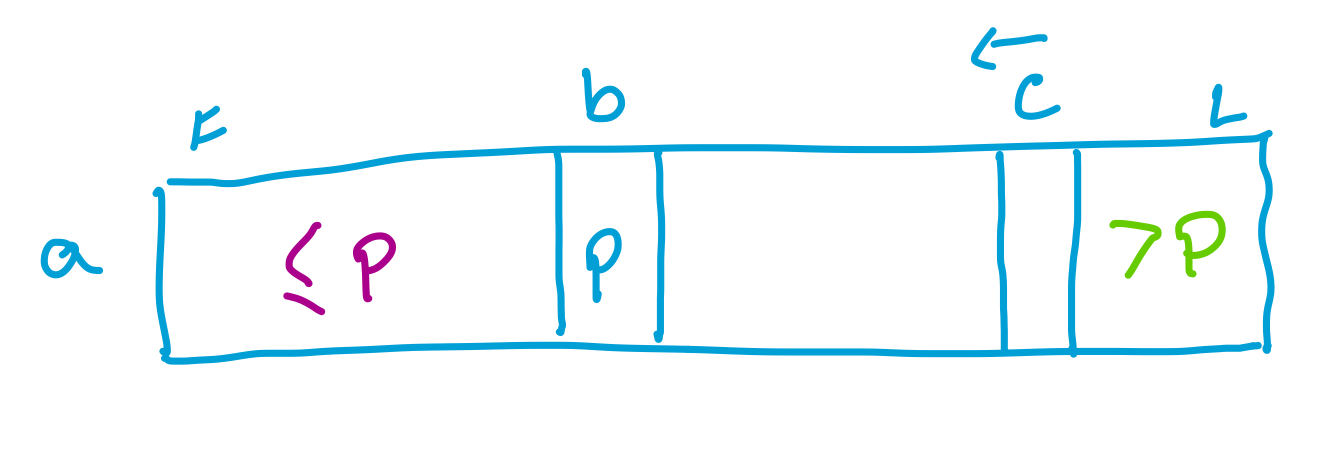
\includegraphics[width=0.6\textwidth]{alt_pivot_invariant.jpeg}
\end{center}

This gave me the insight I needed.  My algorithm is:
\begin{enumerate}
\item starting from $F$, move $b$ to the right as long as the value is increasing.  I.e. if you have $[1,2,3,2,4]$, stop at the $3$.
\item Now inspect the value at $c$.  If it is greater than $p$, decrement $c$.  If it is less than or equal to $p$ then swap $b$ with $b+1$, swap $b$ with $c$, and increment $b$.
\item Stop when $c == b$.
\end{enumerate}

Coding this up is a fun exercise and you can use this version in place of any other partition algorithms, they are interchangeable if you write your overall pivot function appropriately.

\section{Quick Sort: Alternative Domain}

I drew a diagram of the hint to help me

\begin{center}
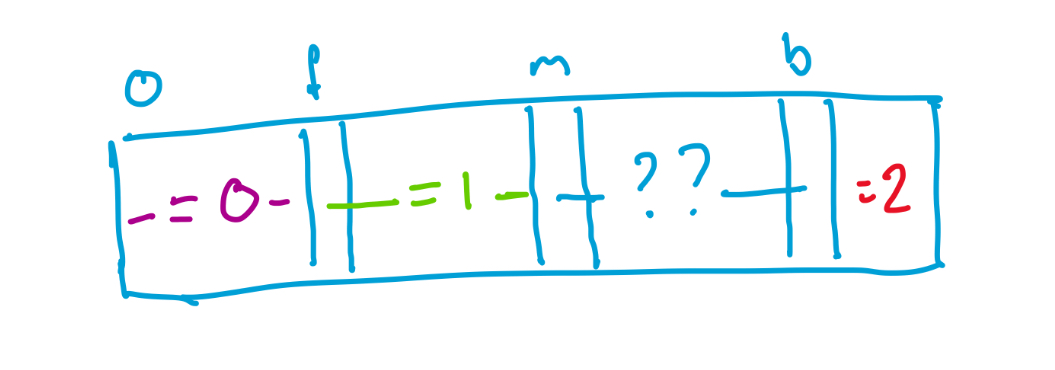
\includegraphics[width=0.6\textwidth]{three_value_sort.jpeg}
\end{center}

From that I can tell that $f$ and $m$ need to start at $0$ and $b$ needs to start at $N-1$.  Then I just inspect the next element in the unknown region and decide where it belongs.  I can do the right swaps to get it there, and move on!  Here is my code to do that.

{\small
\begin{lstlisting}[language=java]
char[] threeValueSort(char[] a){
    int f = 0;
    int m = 0;
    int b = a.length-1;
    while (b >= m){
        char curr = a[b];
        if (curr == '0'){
            swap(a, f, m);
            swap(a, f, b);
            f++;
            m++;
        } else if(curr == '1'){
            swap(a, b, m);
            m++;
            b--;
        } else {
            b--;
        }
    }
    return a;
}

@Test
public void testThreeValue(){
    assertArrayEquals(threeValueSort(new char[] {}), 
                                     new char[]{});
    assertArrayEquals(threeValueSort(new char[] {'1'}), 
                                     new char[]{'1'});
    assertArrayEquals(threeValueSort(new char[] {'2','1'}), 
                                     new char[]{'1','2'});
    assertArrayEquals(threeValueSort(new char[] {'2','1','0'}), 
                                     new char[]{'0','1','2'});
    assertArrayEquals(threeValueSort(new char[] {'2','1','0','1'}), 
                                     new char[]{'0','1','1','2'});
    assertArrayEquals(threeValueSort(new char[] {'0','1','0'}), 
                                     new char[]{'0','0','1'});
}
\end{lstlisting}
}

\section{Quick Sort: Search}

If the partition algorithm returned the final position of the pivot ($p$), I could use this to make it into a binary search.  The key "trick" is that once a pivot item is set, it won't move. So if it ends up in the k'th position then we know for sure it will end up as the k'th item.
\begin{description}
\item [$p = k$] We know we have found the k'th smallest item.
\item [$p < k$] We only need to search in the top "half".
\item [$p > k$] We only need to search in the bottom "half".
\end{description}

Note that, just like quicksort, this has good average and best case speed, but the worst case speed is still $O(n)$ (just like a boring linear search).

\section{Stability}
Merge Sort is stable, Quick Sort is not.  You can see it by going back to the traces.  Equal elements don't ever get swapped about in merge sort but they could in the quick sort partition.

\end{document}